\subsection{Chromatogram of Barley Flour}
\begin{figure}[h]
    \centering
    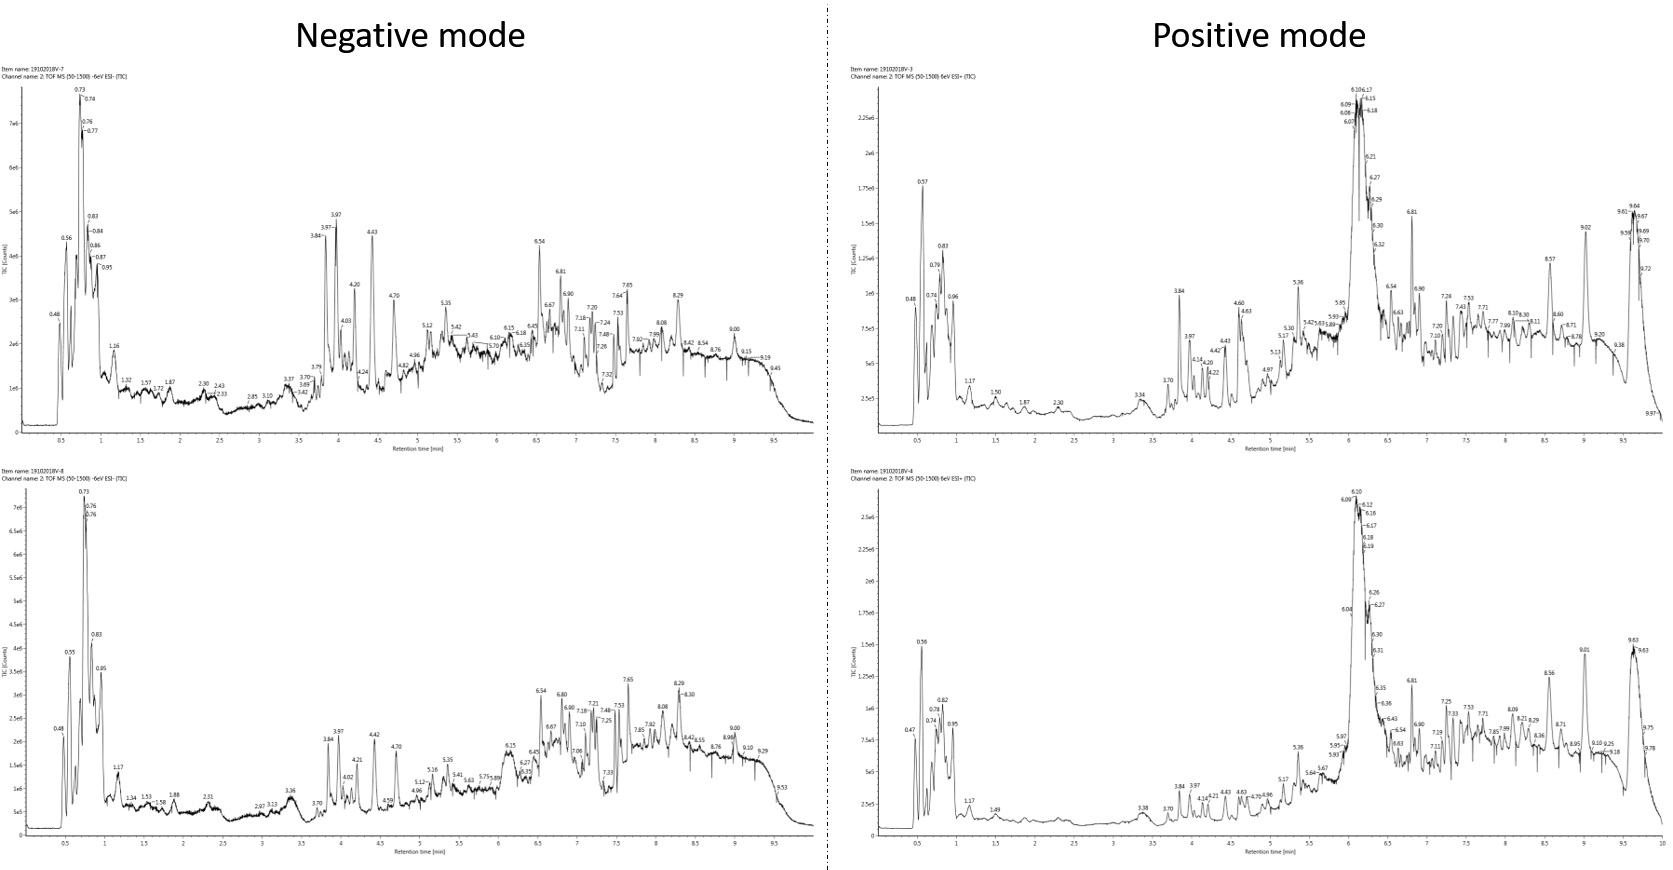
\includegraphics[scale=0.4]{images/chromatogram_barley_1.png}
    \caption{Chromatogram of Barley Flour (from top to the bottom: bran flour and endosperum flour)}
    \label{fig:chromatogram_barley}
\end{figure}

\clearpage
\subsection{\acrfull{ms/ms} spectra of phytosterols}
\acrshort{ms/ms} spectra of common phytosterols are shown in Figure \ref{fig:sterolmsms}, adapted from \cite{sterolms}
\begin{figure}[H]
    \centering
    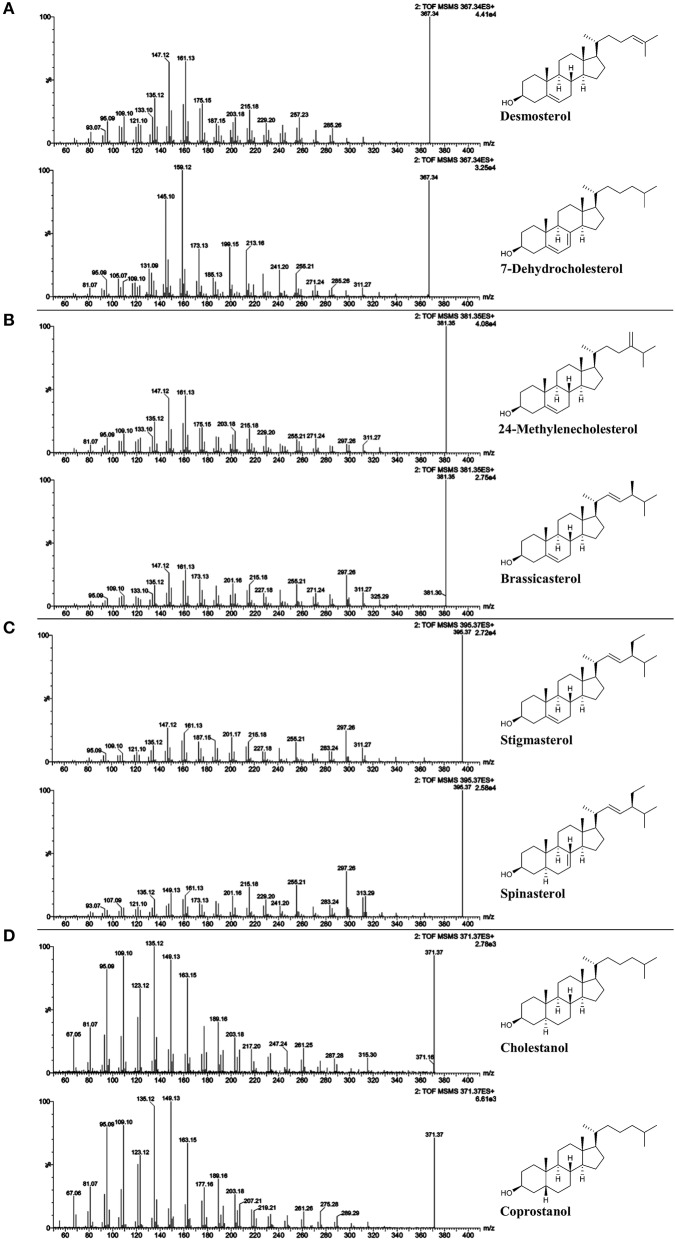
\includegraphics[scale=1]{images/sterolmsms.jpg}
    \caption{\acrshort{ms/ms} spectra of common phytosterols}
    \label{fig:sterolmsms}
\end{figure}